\documentclass{mc2015}



\usepackage{amsmath}
\usepackage{amssymb}
\usepackage{amsthm}
\usepackage{amscd}
\usepackage{amsfonts}
\usepackage{graphicx}%
\usepackage{fancyhdr}
\usepackage{color}
\usepackage{cite}

%\usepackage[T1]{fontenc}
\usepackage[utf8]{inputenc}
\usepackage{authblk}
\usepackage{physics}
\usepackage{float}
\usepackage{caption}
\usepackage{subcaption}

%----------------------ANS TEMPLATE STUFF-------------------------------------------------%
\usepackage[T1]{fontenc}         % Use T1 encoding instead of OT1
\usepackage[utf8]{inputenc}      % Use UTF8 input encoding
\usepackage{microtype}           % Improve typography
\usepackage{booktabs}            % Publication quality tables
%\usepackage{amsmath}
%\usepackage{graphicx}
%\usepackage{float}
\usepackage[exponent-product=\cdot]{siunitx}
\usepackage[colorlinks,breaklinks]{hyperref}
\hypersetup{linkcolor=black, citecolor=black, urlcolor=black}
\usepackage{lipsum}
\def\equationautorefname{Eq.}
\def\figureautorefname{Fig.}
\authorHead{Paul W. Talbot, CongJian Wang, Cristian Rabiti, Anil K. Prinja}
\shortTitle{Collocation for UQ in Nuclear Engineering}


\newcommand{\expv}[1]{\ensuremath{\mathbb{E}[ #1]}}
\newcommand{\xs}[2]{\ensuremath{\Sigma_{#1}^{(#2)}}}
\newcommand{\intO}{\ensuremath{\int\limits_{4\pi}}}
\newcommand{\intz}{\ensuremath{\int\limits_0^1}}
\newcommand{\intf}{\ensuremath{\int\limits_{-\infty}^\infty}}
\newcommand{\intzf}{\ensuremath{\int\limits_{0}^\infty}}
\newcommand{\LargerCdot}{\raisebox{-0.25ex}{\scalebox{1.2}{$\cdot$}}}

%\textwidth6.6in
%\textheight9in


%\setlength{\topmargin}{0.3in} \addtolength{\topmargin}{-\headheight}
%\addtolength{\topmargin}{-\headsep}

%\setlength{\oddsidemargin}{0in}

%\oddsidemargin  0.0in \evensidemargin 0.0in \parindent0em

%\pagestyle{fancy}\lhead{MATH 579 (UQ for PDEs)} \rhead{02/24/2014}
%\chead{Project Proposal} \lfoot{} \rfoot{\bf \thepage} \cfoot{}

\begin{document}
\title{Collocation Methods for Uncertainty Quantification in Nuclear Engineering Applications}

\author{Paul W. Talbot\footnote{paul.talbot@inl.gov}}
\author{CongJian Wang}
\author{Cristian Rabiti}
\author{Andrea Alfonsi}
\author{Joshua Cogliati}
\author{Daniel Maljovec}
\author{Diego Mandelli}
\author{Robert Kinoshita}
\affil{
  Idaho National Laboratory\\ Nuclear System Design and Analysis Division\\ P.O. Box 1625 MS 3870
}

\author{Anil K. Prinja}
\affil{University of New Mexico \\
     Department of Nuclear Engineering \\ 209 Farris Engineering Center \\ Albuquerque, NM 87131}
\maketitle

\begin{abstract}
  TODO abstract

\emph{Key Words}: Uncertainty Quantification, Stochastic Collocation, HDMR, Sparse Grid
\end{abstract}

%\begin{document}
\graphicspath{../graphics}

%\section{Introduction}
% Chapter 1

\chapter{Introduction} % Main chapter title

\label{ch:intro} % For referencing the chapter elsewhere, use \ref{Chapter1} 

\lhead{1. \emph{Introduction}} % This is for the header on each page - perhaps a shortened title

%----------------------------------------------------------------------------------------

%\section{Welcome and Thank You}

%problem description
In simulation modeling, we attempt to capture the behavior of a physical system by describing it in a series
of equations, often partial differential equations.  These equations may be time-dependent, and capture
physics of interest for understanding the system.  A \emph{solver} is then written that can solve the series
of equations and determine quantities of interest (QoI).  A traditional solver accepts a set of inputs and
produces a set of single-valued outputs.  For instance, a solver might solve equations related to the
attenuation of a beam of photons through a material, and the QoI might be the strength of the beam exiting the
material.  A single run of the solver usually results in a single value, or realization, of the quantity of
interest.

This single realization might be misleading, however.  In most systems there is some degree of uncertainty in
the input parameters to the solver.  Some of these uncertainties may be epistemic, or systematic uncertainty
originating with inexact measurements or measurable unknowns.  Other uncertainties might be aleatoric,
intrinsic uncertainty in the system itself, such as probabilistic interactions or random motion.  Taken
together, the input parameter uncertainties exist within a multidimensional probabilistic space.  While some
points in that space may be more likely than others, the possible range of values for the QoI is only
understood when the uncertain input space is considered as a whole.  We note here that while it is possible
that some of the input parameters are correlated in their probabilistic distribution, it is also possible to
decouple them into uncorrelated variables.  Throughout this work we will assume the input parameters 
are uncorrelated.

%Monte Carlo
One traditional method for exploring the uncertain input space is through random sampling, such as in analog Monte
Carlo sampling.  In this method, a point in the input space is chosen at random based on probability.  This
point represents values for the input parameters to the solver.  The solver is executed with these inputs, and
the QoIs are collected.  Then, another point in the input space is chosen at random.  This process continues
until the properties of the QoIs, or \emph{response}, are well understood.

There are some beneficial properties to random sampling approaches like Monte Carlo.  
Significantly, they are unintrusive:
 there is no need to modify the solver in order to use these methods.  This allows a framework of
algorithms to be developed which know only the input space and QoI of a solver, but need no further knowledge
about its operation.  Unintrusive methods are desirable because the uncertainty quantification algorithms can
be developed and maintained separately from the solver.

Monte Carlo and similar sampling strategies are relatively slow to converge on the response surface.  For
example, with Monte Carlo sampling, in order to reduce the standard error of the mean of the response by a factor
of two, it is necessary to take at least four times as many samples.  If a solver is sufficiently computationally
inexpensive, running additional solutions is not a large concern; however, for lengthy and expensive solvers,
it may not be practical to obtain sufficient realizations to obtain a clear response.

% expensive solvers need low-sample UQ
In this work, we will assume solvers are computationally expensive, requiring many hours per solve, and that
computational resource availability requires as few solves as possible.  As such, we consider several methodologies 
for quantifying the uncertainty in expensive solver
calculations.  In order to demonstrate clearly the function of these methods, we apply them first on
several simpler problems, such as polynomial evaluations and analytic attenuation.  These models have a high
degree of regularity, and their analyticity provides for straightforward benchmarking.  Through gradual
increasing complexity, we investigate the behavior of the UQ methods.

Finally, we apply the methods to an engineering-scale solver that
models the neutronics and performance of nuclear fuel.  This will
demonstrate the practical application of the uncertainty quantification methods, where the regularity and
other properties of the model are not well understood.

The first uncertainty quantification method we consider
is traditional analog Monte Carlo (MC) analysis, wherein random sampling of the input space generates a view of
the response.  MC is used as a benchmark methodology; if other methods converge on moments of the quantities
of interest more quickly and consistently than MC, we consider them ``better'' for our purposes.

The second method we consider is stochastic collocation for generalized polynomial
chaos (SCgPC)\cite{sparseSC,sparse1,sparse2,xiu}, whereby deterministic collocation points 
are used to develop a polynomial-interpolated reduced-order model
of the response as a function of the inputs.  This method algorithmically expands the solver as the sum of
orthogonal multidimensional polynomials with scalar coefficients.  The scalar coefficients are obtained by
numerical integration using multidimensional collocation (quadrature) points.  The chief distinction between
SCgPC and Monte Carlo methods is that SCgPC is deterministic, in that the realizations required from the
solver are predetermined instead of randomly sampled.  There are two major classes of deterministic
uncertainty quantification methods: intrusive and unintrusive.  Like Monte Carlo, SCgPC is unintrusive
and performs well without any need to access the operation of the solver.  This behavior is desirable for
construction black-box approach algorithms for uncertainty quantification.  Other intrusive methods such as
stochastic Galerkin exist \cite{galerkin}, but require solver modification to operate.  This makes them
solver-dependent and undesirable for an independent uncertainty quantification framework.

The other methods we present here expand on
SCgPC.  First, we introduce non-tensor-product methods for determining the set of polynomial bases to
use in the expansion.  Because a tensor product grows exponentially with increasing cardinality of the input
space, we combat this curse of dimensionality using the 
alternative polynomial set construction methods\cite{hctd}.
These bases will then be used to construct Smolyak-like sparse grids \cite{smolyak} to provide collocation
points that in turn calculate the coefficients in the polynomial expansion.  Second, we consider
anisotropic sparse grids,
allowing higher-order polynomials for particular input parameters.  We also consider methods for
obtaining weights that determine the level of anisotropic preference to give parameters, and explore the effects of a
variety of anisotropic choices.

The second method group we consider is high-dimension model representation (HDMR), which correlates with Sobol
decomposition \cite{hdmr}.  This method is useful both for developing sensitivities of the quantity of interest to subsets
of the input space, as well as constructing a reduced-order model itself.  We demonstrate the strength of HDMR
as a method to inform anisotropic sensitivity weights for SCgPC.

Finally, we consider adaptive algorithms to construct both SCgPC and HDMR expansions using second-moment
convergence criteria.  We analyze these for potential efficiencies and shortcomings.  We also propose future
work to further improve the adaptive methods.

We implement all these methods in Idaho National Laboratory's \raven{}\cite{raven}
uncertainty quantification framework. \raven{} is a Python-written framework that non-intrusively provides
tools for analysts to quantify the uncertainty in their simulations with minimal development.  To demonstrate
the application of the method developed, we use a complex non-linear multiphysics system solver simulating
the operation of a fuel pin within a nuclear reactor core, including both neutronics and fuel performance
physics kernals.  For this solver, we use the coupled \rattlesnake{}\cite{rattlesnake} and 
\bison{} \cite{bison,mammoth} production codes.
Both of these codes are developed and maintained within the \moose{}\cite{moose} environment.  The
multiphysics nonlinear system provides a challenge with unknown response properties for the uncertainty
quantification methods discussed in this proposal.

%outline chapters
The remainder of this work will proceed as follows:
\begin{itemize}
  \item Chapter 2: We describe the analytic test problems and engineering-scale problem solved by the simulations 
    we will be running, along with their properties and inferences about the algorithms developed.
    We discuss potential approaches to model solving and applications of the models.
  \item Chapter 3: We describe methods for uncertainty quantification, including Monte Carlo (MC),
    stochastic collocation for generalized Polynomial Chaos (SCgPC), and high-dimension model reduction
    (HDMR).  We additionally describe adaptive methods for SCgPC and HDMR.
  \item Chapter 4: We analyze results obtained for the various UQ methods on analytic models, and contrast 
    them with traditional Monte Carlo convergence on statistical moments.
  \item Chapter 5: We perform analysis on the engineering-scale multiphysics coupled problem, and analyze
    results.
  \item Chapter 6: We consider application of collocation-based methods to time-dependent sensitivity analysis.
  \item Chapter 7: We draw conclusions from the evaluations performed, and offer some suggestions for
    applicability and limitations discovered.
  \item Chapter 8: We consider new research and future development uncovered by the UQ methods demonstrated here.
\end{itemize}
%----------------------------------------------------------------------------------------


%\section{Methods}
% Chapter Template

\chapter{Methods} % Main chapter title

\label{Chapter3} % Change X to a consecutive number; for referencing this chapter elsewhere, use \ref{ChapterX}

\lhead{Chapter 3. \emph{Methods}} % Change X to a consecutive number; this is for the header on each page - perhaps a shortened title

%----------------------------------------------------------------------------------------
%	SECTION: INTRO
%----------------------------------------------------------------------------------------

\section{Todo}
todo.


%\section{Implementation}
\section{Implementation}
TODO implementation in RAVEN
\begin{itemize}
  \item PCA
  \item Sampler/ROM connection
  \item Adaptive methods
\end{itemize}


%\section{Results}
% Chapter Template

\chapter{Preliminary Results} % Main chapter title

\label{ch:results} % Change X to a consecutive number; for referencing this chapter elsewhere, use \ref{ChapterX}

\lhead{Chapter 4. \emph{Results}} % Change X to a consecutive number; this is for the header on each page - perhaps a shortened title

We consider some results from applying the methods described in Chapter \ref{ch:methods} to the physical
models outlined in Chapter \ref{ch:models}, organized by model.
%----------------------------------------------------------------------------------------
%	SECTION 1
%----------------------------------------------------------------------------------------

\section{Polynomial Evaluations}
Using an analytic polynomial evaluation as our model allows observation of SCgPC performance for
multiple dimension cardinalities.  Uniformly distributing the input parameters from 0 to 1, the mean and variance are
\begin{align}
  \text{mean}&=\left(\frac{3}{2}\right)^N,\\
  \text{var}&=\left(\frac{7}{3}\right)^N-\left(\frac{3}{2}\right)^{2N},
\end{align}
where $N$ is the cardinality of the input space.  As seen in Figures \ref{fig:anl5_varconv} and
\ref{fig:anl10_varconv}, the increase in dimensionality has great impact on the convergence rate of SCgPC
methods.  There are several
inferences that we make using these results. In the figures, the following abbreviations are used:
\begin{itemize}
  \item \emph{mc}: Monte Carlo traditional sampling,
  \item \emph{tp}: Tensor Product-based SCgPC,
  \item \emph{td}: Total Degree-based SCgPC,
  \item \emph{hc}: Hyperbolic Cross-based SCgPC,
  \item \emph{adapt}: Adaptive SCgPC.
\end{itemize}

First, we note the tensor product (tp) method for polynomial basis set construction is an outlier, in that
with 200 computational solves the error is already converged to 11 orders of magnitude.  This is because of
the model being solved; it is, in effect, a tensor product of first-order polynomials.  For this particular
model, the tensor product method should be ideally efficient.  It is omitted in Fig.
\ref{fig:anl10_varconv} for clarity.

Second, we note that the two other static polynomial index sets, total degree (td) and hyperbolic cross (hc)
perform similarly well and converge faster than traditional Monte Carlo.  In the case of total degree, some
exponential convergence is observed, while it is unclear if hyperbolic cross is linear or exponential.  We
also note the strong dependence of SCgPC on input dimension cardinality for efficient convergence.

Finally, for this case we
also present some preliminary results for the Adaptive SCgPC method.  While it performs remarkably well for
the five-dimension problem, it stalls for the ten-dimension problem.  This is likely because of the
computational costs in searching the polynomial space.  Because of the tensor-first-order nature of the model,
the predictive algorithm behind Adaptive SCgPC incorrectly predicts that terms containing second-order
polynomials in any dimension are more significant than terms containing higher-interactivity first-order
polynomials.  Because of this, the Adaptive SCgPC method spends considerable effort in unproductive searching.

\begin{figure}[H]
  \centering
    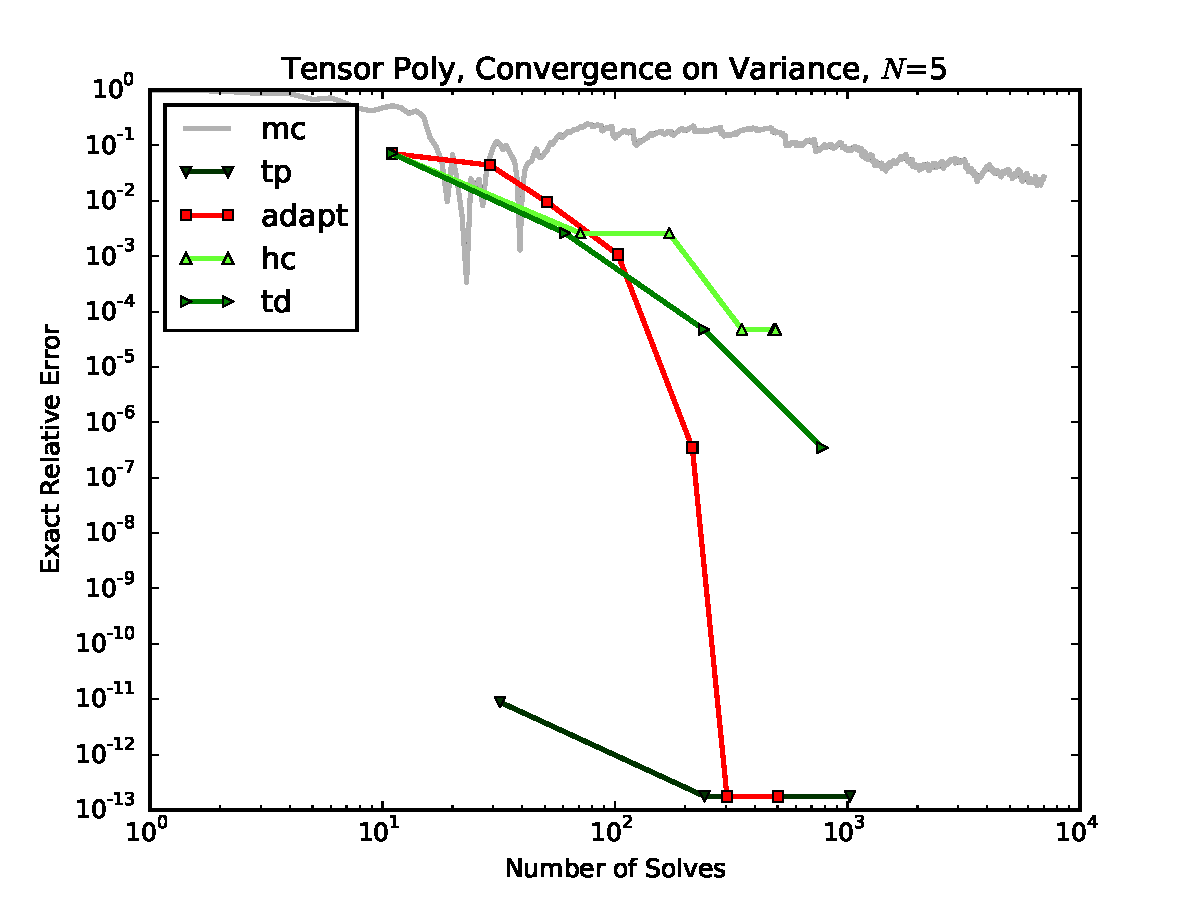
\includegraphics[width=0.7\linewidth]{tenspoly_varconv_5}
    \rule{35em}{0.5pt}
  \caption{Analytic $N=5$ Error Convergence, Variance}
  \label{fig:anl5_varconv}
\end{figure}
\begin{figure}[H]
  \centering
    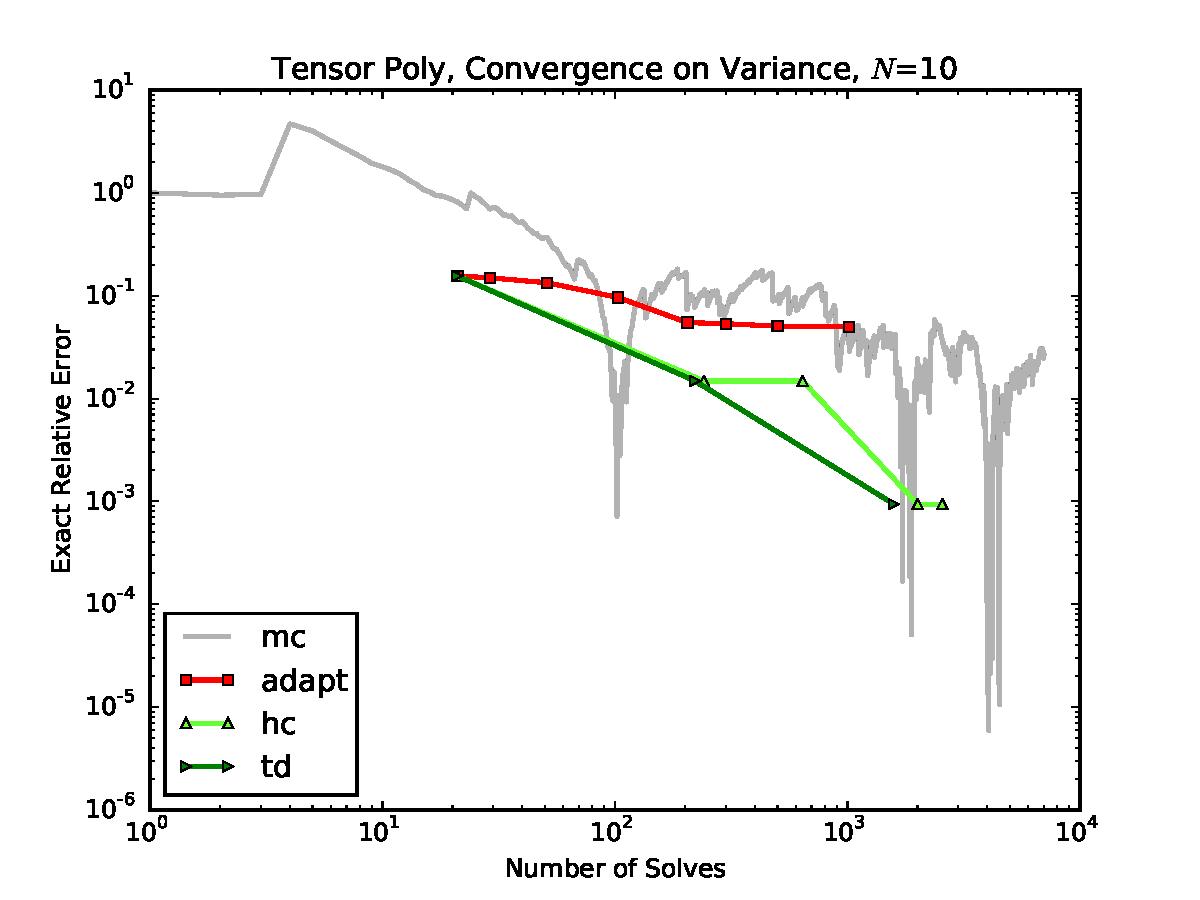
\includegraphics[width=0.7\linewidth]{tenspoly_varconv_10}
    \rule{35em}{0.5pt}
  \caption{Analytic $N=10$ Error Convergence, Variance}
  \label{fig:anl10_varconv}
\end{figure}



\section{Attenuation}
Similar to the polynomial model, the attenuation model does not converge exactly for any order of SCgPC
expansion, as exponential terms cannot be perfectly represented by a finite sum of polynomials.
Again distributing the input variables from 0 to 1, the mean and variance are
\begin{align}
  \text{mean}&=N^N\left(1-\exp(-\frac{1}{N})\right)^N,\\
  \text{var}&=\left(\frac{N}{2}\right)^N \left(1-\exp(-\frac{2}{N})\right)^N - \text{mean}^2,
\end{align}
where $N$ is the cardinality of the input space.  The convergence plots are shown in Figs.
\ref{fig:att5_varconv} and \ref{fig:att10_varconv}.

While considering this model, it is useful to expand the solution in a Taylor series for polynomial behavior.
In any one dimension,
\begin{equation}
  e^{-x} = 1 - x + \frac{x^2}{2!} - \frac{x^3}{3!} + \mathcal{O}(x^4).
\end{equation}
Because $y_n\in[0,1]$ and the nature of the polynomial expansion, we expect leading, low-order polynomial
terms to dominate the SCgPC expansion, and interactivity to be more dominant than high-order polynomials,
somewhat like the Polynomial Evaluations case above.

There are several notable features in this convergence graph that are not seen in the tensor polynomial case.
First, the Tensor Product and Total Degree index sets are very similar in exponential convergence; this is
somewhat expected given the polynomial expansions above.  Neither Total Degree nor Tensor Product ideally fit
this model as a low-order expansion, but both cover critical components of it as they grow in size.

The convergence of the Hyperbolic Cross index set is possibly the most striking result here.  The oscillatory
nature of the solutions covers a band wide enough to disguise any convergence after 100 computational solves.
It appears that the behavior is due to poor integration of high-order polynomial coefficients.  When a
polynomial is first added to the index set, insufficient quadrature is used to integrate the coefficient,
resulting in a large error for that coefficient.  However, when further points are added, the
poorly-integrated coefficient is resolved, and the variance converges more closely.  This behavior warrants
more investigation.

Lastly, we see some plateau behavior for the Adaptive SCgPC method. TODO WORKING XXX



Interestingly, while the convergence of the adaptive method seems to be converging at a better rate than the
total degree isotropic set, there is no clear advantage for up to thousands of solves.  This is somewhat
expected, as there is coupling between inputs evident in the Taylor expansion of the attenuation model.  
As with the polynomial model,
the curse of dimensionality is clear.

\begin{figure}[H]
  \centering
    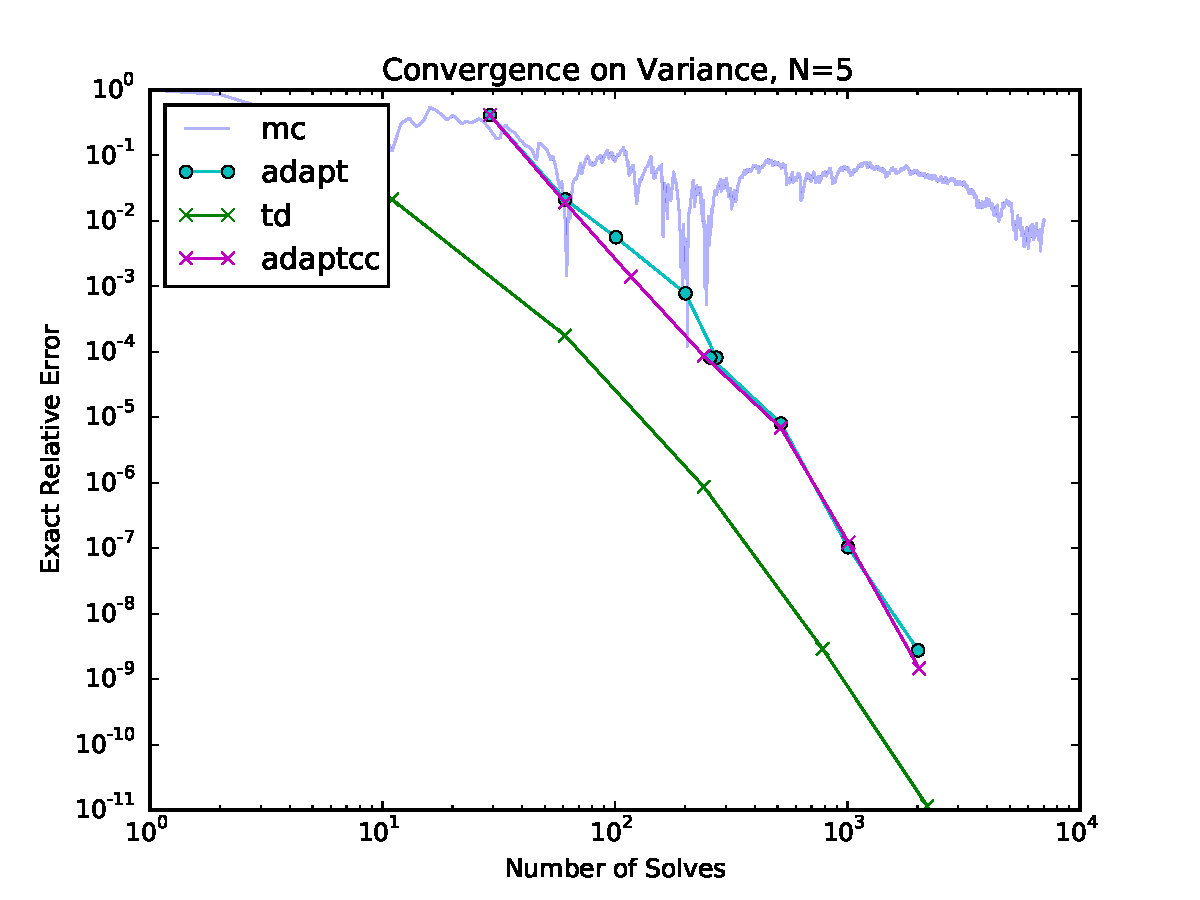
\includegraphics[width=0.7\linewidth]{attn_varconv_5}
    \rule{35em}{0.5pt}
  \caption{Attenuation $N=5$ Error Convergence, Variance}
  \label{fig:att5_varconv}
\end{figure}

\begin{figure}[H]
  \centering
    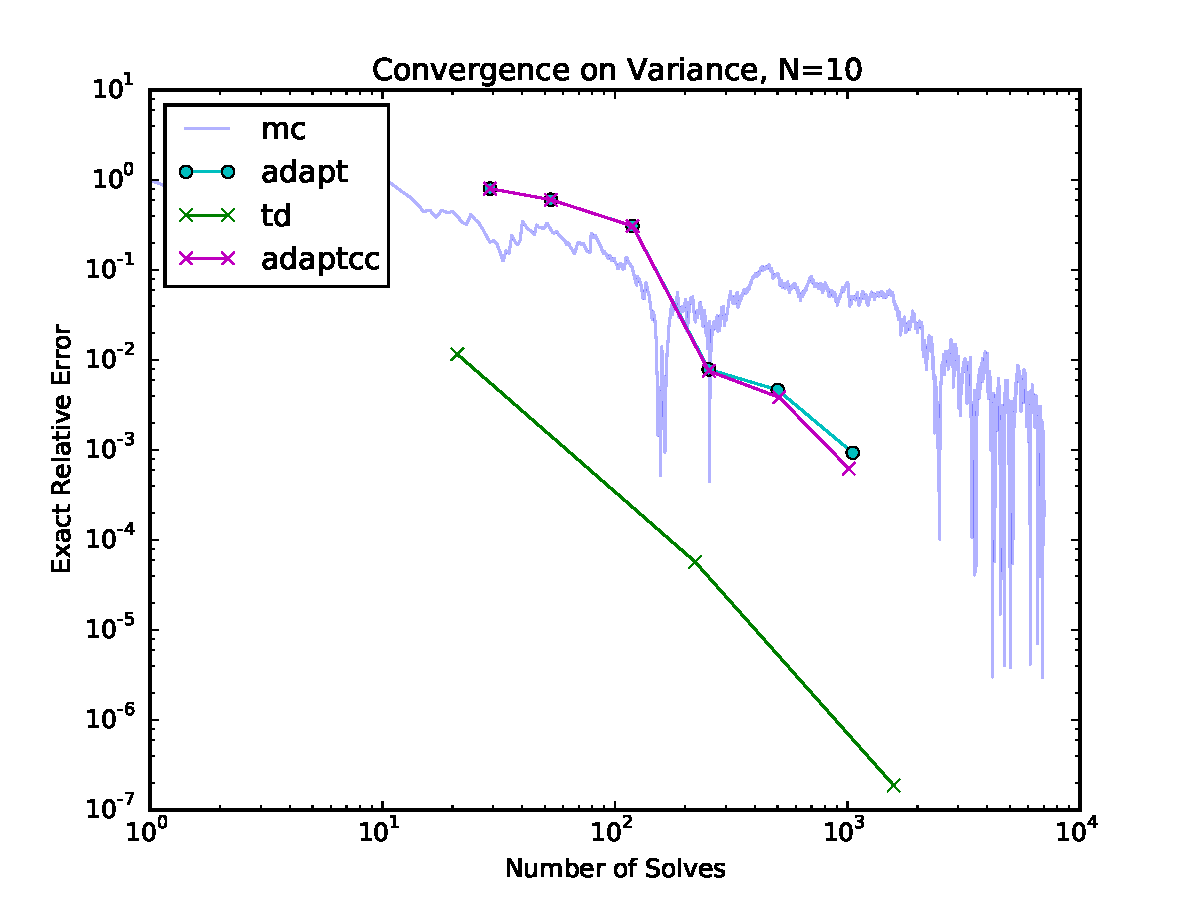
\includegraphics[width=0.7\linewidth]{attn_varconv_10}
    \rule{35em}{0.5pt}
  \caption{Attenuation $N=10$ Error Convergence, Variance}
  \label{fig:att10_varconv}
\end{figure}



\section{Projectile}
Unlike the attenuation and polynomial models, the projectile model is a nonlinear problem without an analytic
solution.  As a result, the convergence benchmark is one achieved by a large Monte Carlo run, instead of an
analytic benchmark; thus, the convergence of the various methods is limited to the convergence of the Monte
Carlo point.  The most converged Monte Carlo point for this work is
\begin{align}
  \text{mean} = 1234, \\
  \text{var} = 1234.
\end{align}
Additionally, this is the first model where significant anisotropy exists in the model.  For instance, the
drag coefficient parameter is many orders of magnitude more influential on the quantity of interest than the
gravitational acceleration.  
The results in Fig. \ref{fig:proj_varconv} are interesting, and require additional data points to understand
clearly.  However, we include Fig. \ref{fig:proj_varval} for clarity.  While it initially looks like the adaptive
methods converge quickly, it appears that this is misleading, as shown in the values graph.  The adaptive
method is converging, but passes through the benchmark value before turning back to converge on it.  This
indicates the adaptive construction introduces too much variance initially, and additional terms are required
to approach the benchmark solution.
\begin{figure}[H]
  \centering
    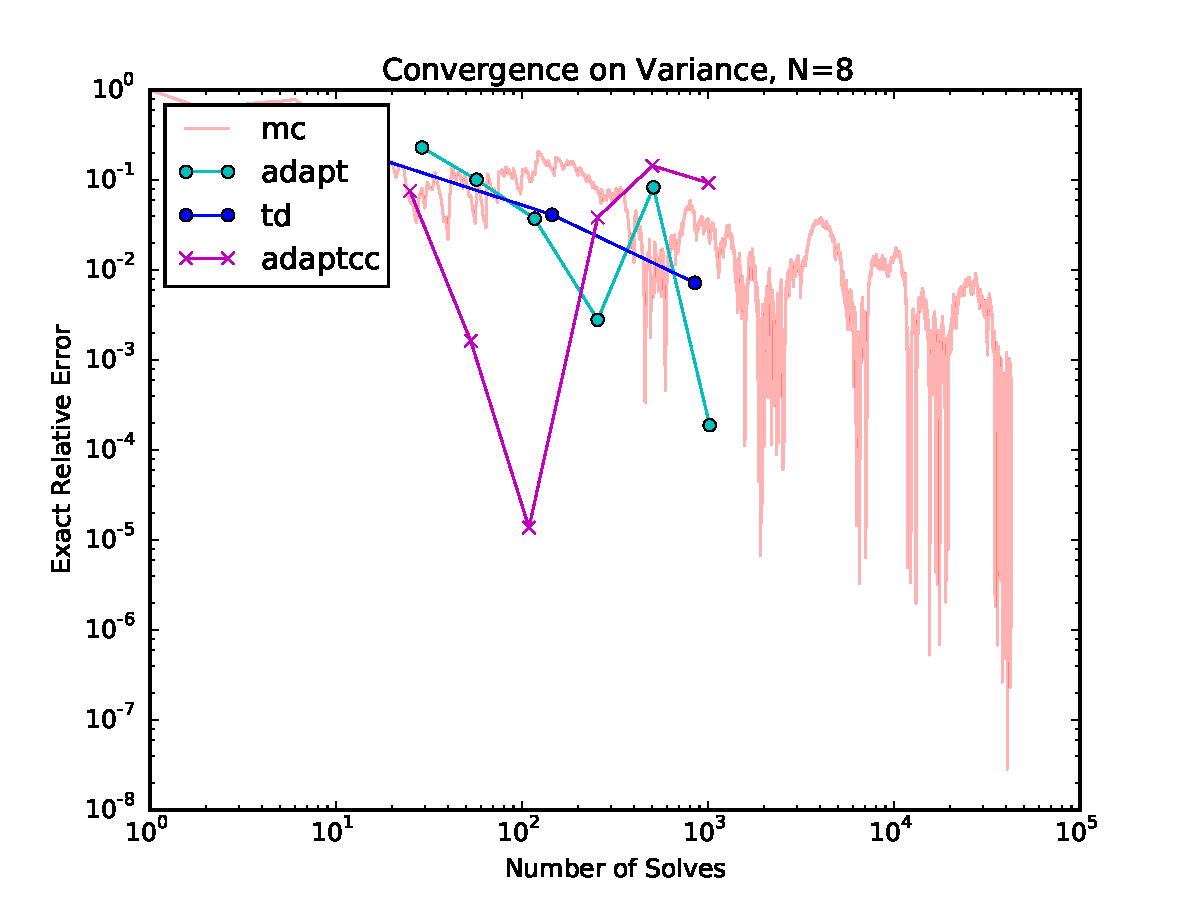
\includegraphics[width=0.7\linewidth]{proj_varconv_8}
    \rule{35em}{0.5pt}
  \caption{Projectile $N=8$ Error Convergence, Variance}
  \label{fig:proj_varconv}
\end{figure}
\begin{figure}[H]
  \centering
    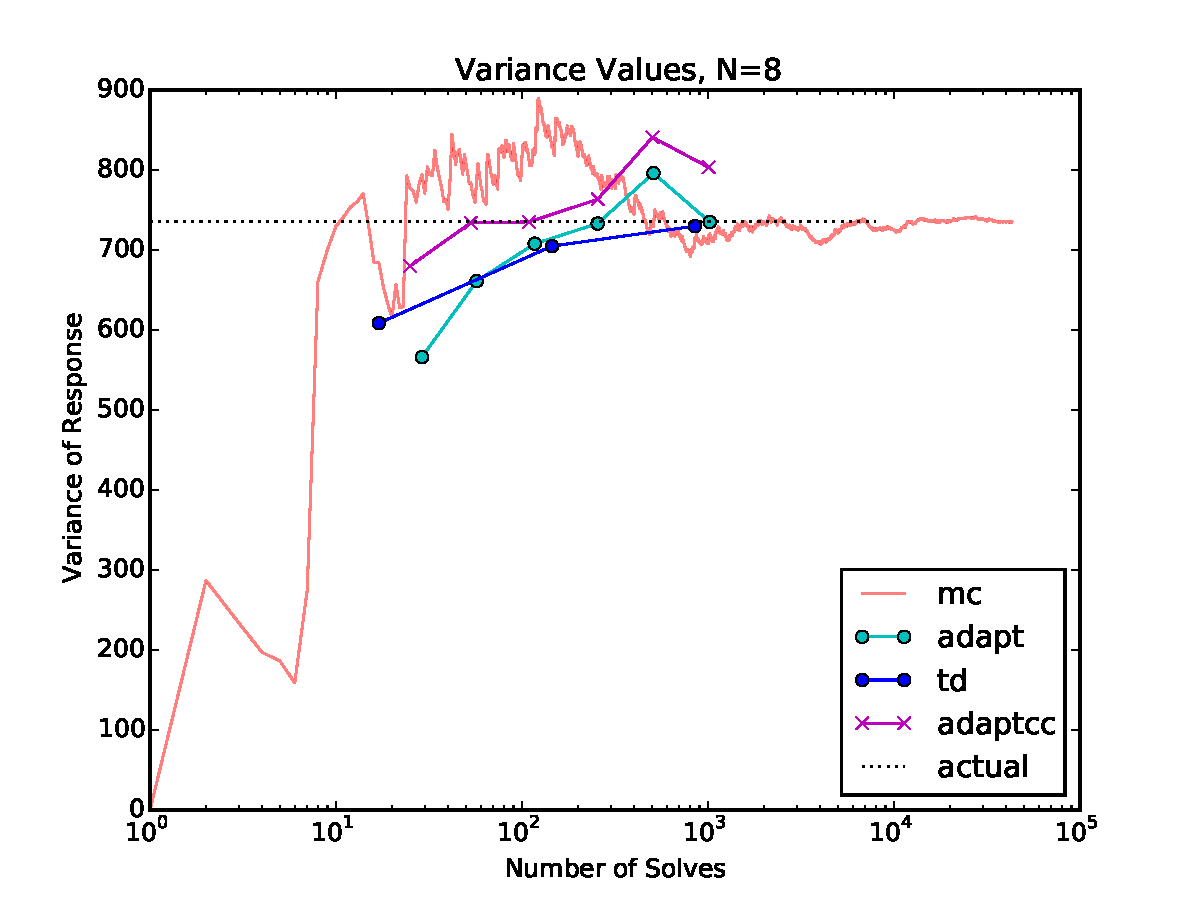
\includegraphics[width=0.7\linewidth]{proj_varvals_8}
    \rule{35em}{0.5pt}
  \caption{Projectile $N=8$ Values, Variance}
  \label{fig:proj_varval}
\end{figure}
%\begin{figure}[H]
% \centering
%   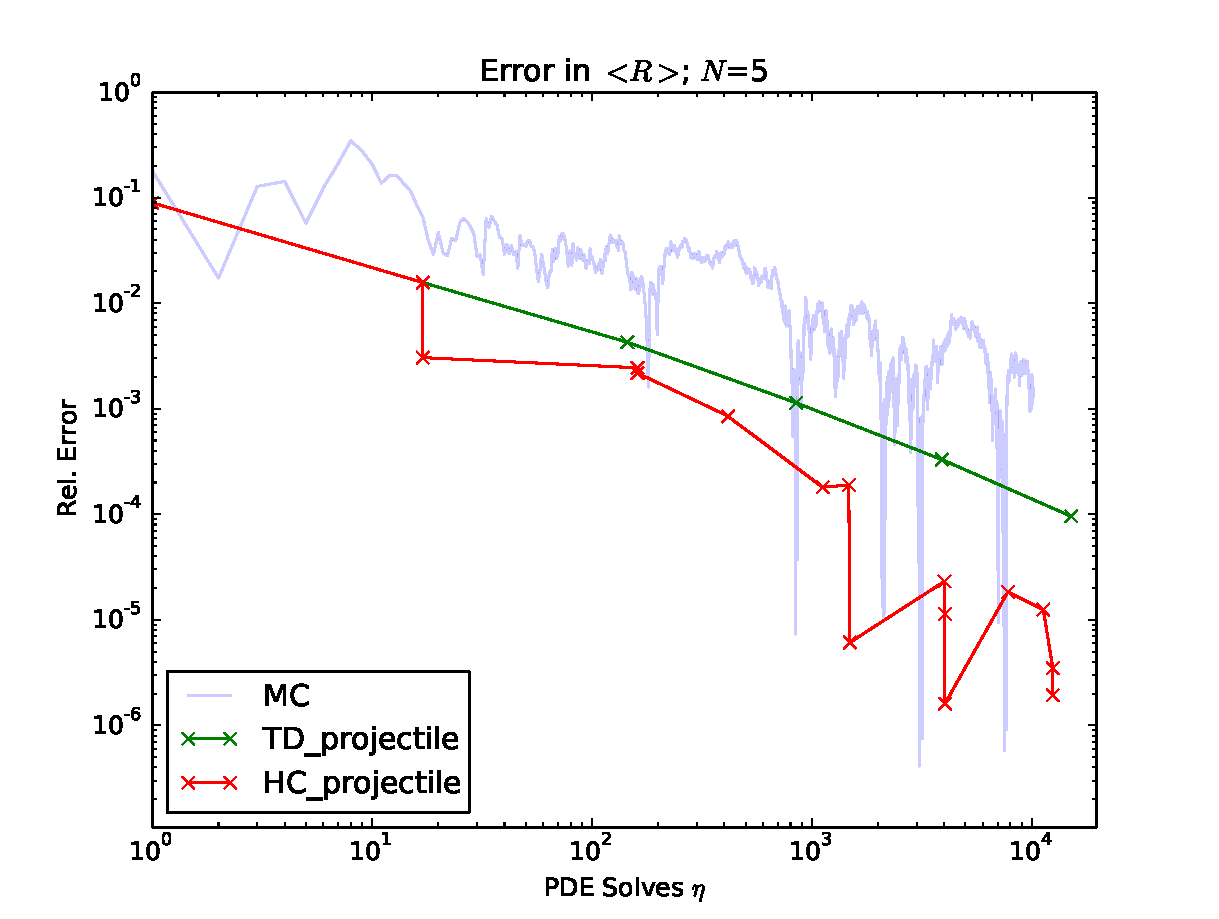
\includegraphics[width=0.7\linewidth]{projectile_errs}
%    \rule{35em}{0.5pt}
%  \caption{Projectile $N=8$ Error Convergence, Variance}
%  \label{fig:proj_varconv}
%\end{figure}



\section{Neutron Diffusion}
The neutron diffusion model is a complex, nonlinear model that begins to approach an engineering-scale model.
Because of complications with conflicting libraries, the adaptive SCgPC method was not available for this
model.  Particularly of note is the clear and obvious loss of convergence rate with increase in the
cardinality of the input space. \{Note to self: fix coloring in plots.\}

\begin{figure}[H]
  \centering
    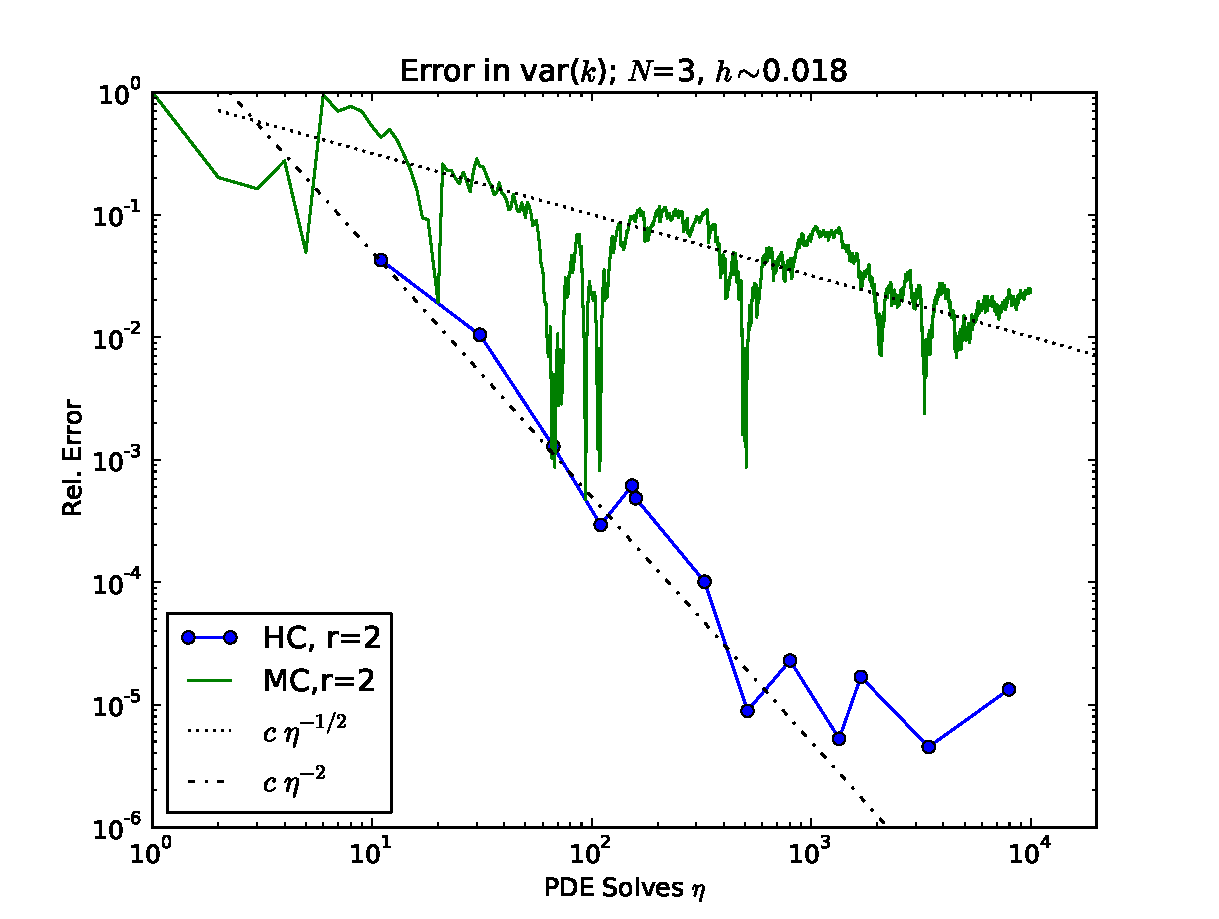
\includegraphics[width=0.7\linewidth]{N3_h5_MCHC_2}
    \rule{35em}{0.5pt}
  \caption{Diffusion $N=3$ Error Convergence, Variance}
  \label{fig:diff3_varconv}
\end{figure}
\begin{figure}[H]
  \centering
    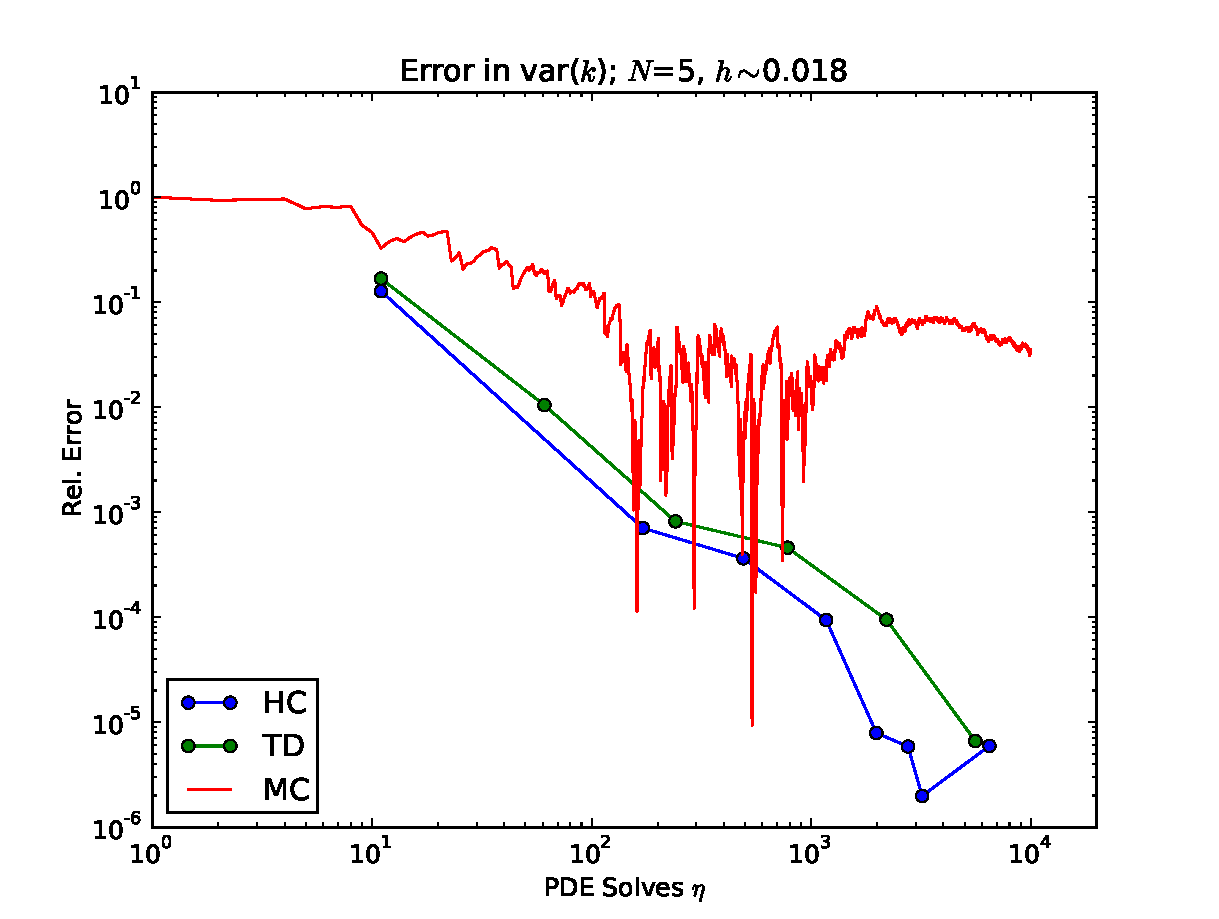
\includegraphics[width=0.7\linewidth]{N5_h5_MCHC_2}
    \rule{35em}{0.5pt}
  \caption{Diffusion $N=5$ Error Convergence, Variance}
  \label{fig:diff5_varconv}
\end{figure}
\begin{figure}[H]
  \centering
    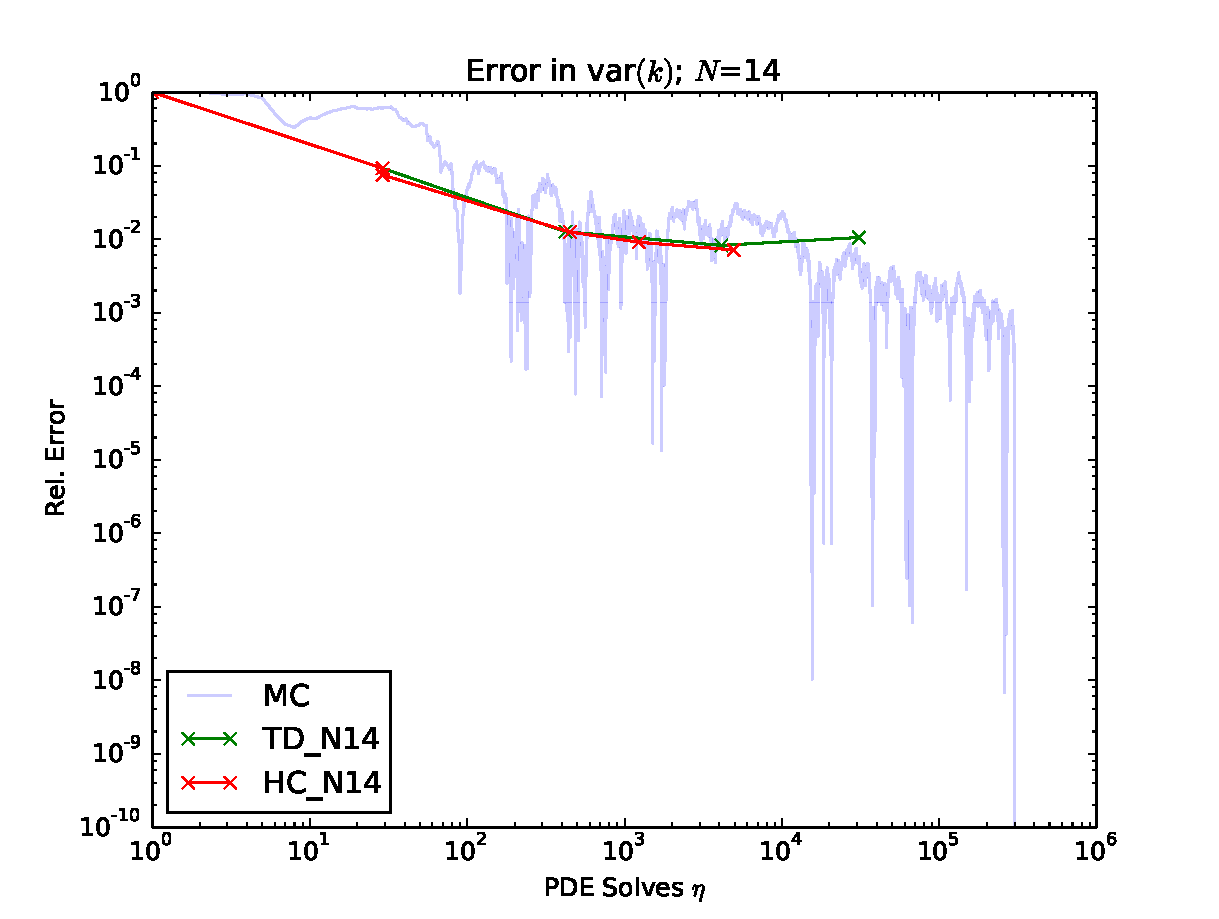
\includegraphics[width=0.7\linewidth]{N14_iso_var_errs}
    \rule{35em}{0.5pt}
  \caption{Diffusion $N=14$ Error Convergence, Variance}
  \label{fig:diff14_varconv}
\end{figure}





\section{Conclusions}
From evaluating the results using the various methods on these models, there are a few useful conclusions.

First, especially for models with small input cardinality, SCgPC methods tend to be faster converging than
traditional Monte Carlo methods.  In particular, the adaptive SCgPC method eventually exhibits exponential
convergence in the models considered here.  This is encouraging for many uncertainty quantification problems
where the variance is chiefly centered on a few input parameters.

%Second, using Clenshaw Curtis quadrature appears to have no negative consequence on converging with the
%adaptive SCgPC method, but no striking positive consequence either.  This suggests it is worth exploring other
%nested quadrature methods that might be beneficial in general, or at least in certain circumstances.

Second, it is clear that even with adaptive SCgPC, convergence is poor for input spaces with at least ten
inputs for less than a thousand solves.  For costly engineering codes, even a thousand runs may be
impractical, so further improvement of the adaptive algorithm is necessary.  This leads to the desirability of
the adaptive HDMR method, which can further subdivide the input domain.  These subdivided domains have
cardinality much more suitable to SCgPC methods.

Lastly, because SCgPC methods improve drastically with decreases in input cardinality, we expect SCgPC to
benefit from coupling with input reduction methods, such as sensitivity-weighted input reduction through
principal component analysis using input-input covariance matrices.


\section{Conclusion}
TODO conclusion

\section{Acknowledgments}
TODO acknowledgements

\setlength{\baselineskip}{12pt}

\bibliographystyle{mc2015}
%\bibliography{references}

%\newpage
\bibliography{../bibliography/uq}
%\bibliographystyle{plain}
\end{document}
